
\begin{figure}[t!]
\centering
\fbox{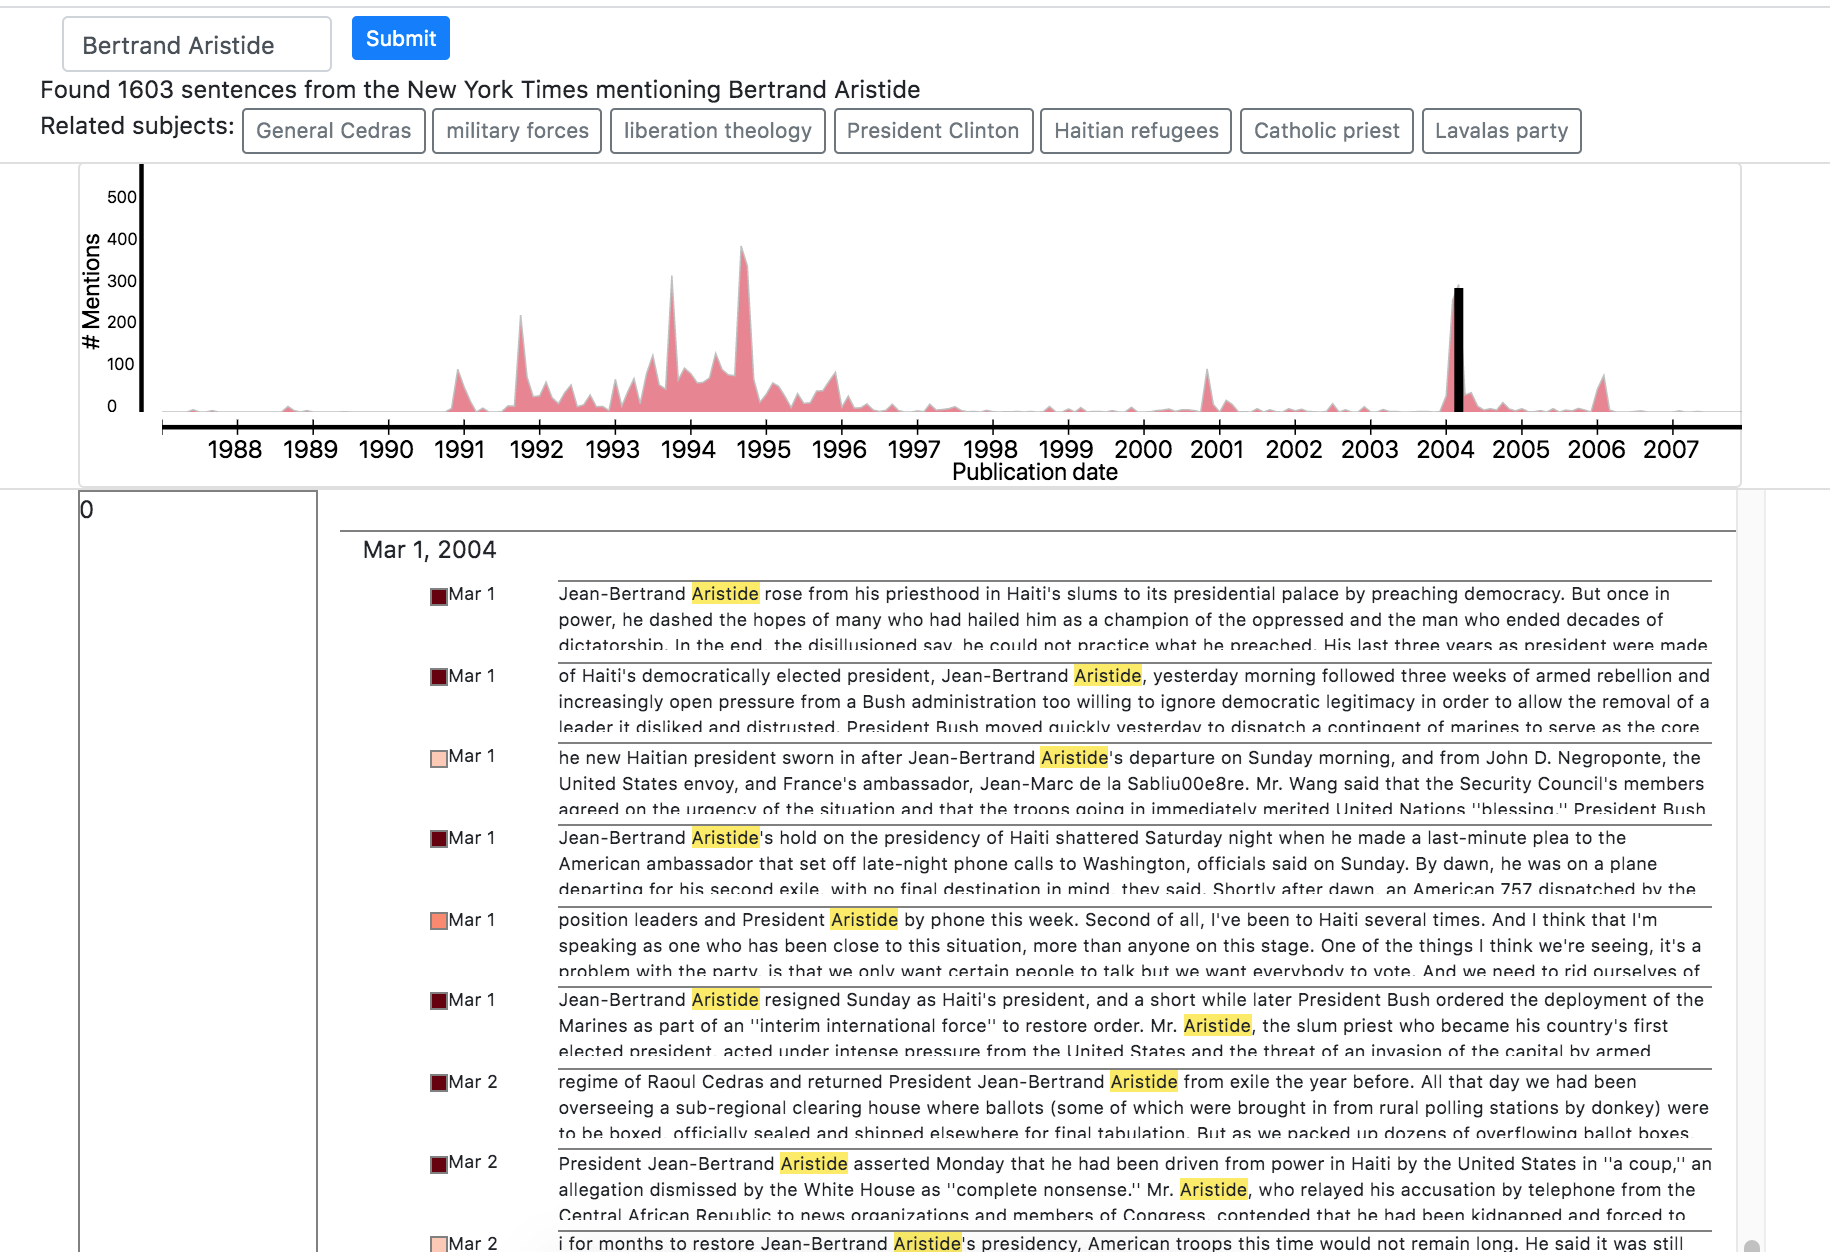
\includegraphics[width=.55\linewidth]{figures/p2.png}}
  \caption[An early prototype of \ours]{  
  An early prototype of \ours, displaying and highlighting every single mention of the query term ``Aristide'' in \textit{New York Times} articles mentioning ``Haiti''. ``Are we showing too much information in this interface?'' one researcher from our group asked \ifour, when presenting the prototype. ``This is literally every mention of your query term.''
\textit{``No this is good},''  \ifour~explained, \textit{``because of what I was calling the type II error concern [i.e.\ the fear of missing relevant material]. When I see something that is trying to decide or curate for me that is a worry. That is a red flag.''} 
However, \ifour~went on to explain how the interface needed to provide more context and transparency surrounding highlighted snippets. 
\textit{``With this design you have to click or read each snippet to see if it is relevant,''} he said.  ``\textit{The snippets are valuable and good but very small and you have to look at the contents of the article. Sometimes you can eliminate that by just quickly scanning the article title ... there needs to be a way to provide the information in a more transparent way.}'' 
(The search bar shown at the top is non-functioning mockup; the ``0'' on the left hand side is a placeholder.)
}\label{f:prototype2}
\end{figure}
